% Hamad Medical Corporation
% Georges Younes

\section{Topological Update Algorithms for Incremental Cutting of 3D Meshes}\label{sec:topological_updates}

One modeling challenge in surgical simulation is the geometric and topological representation of cuts and their effects on an underlying tetrahedral mesh. In this section we describe the data structures and algorithms to address this problem. 

Testing push from github to overleaf.

\subsection{Tetrahedral Subdivision Template}

Cutting a tetrahedral mesh should result in a new tetrahedral mesh retaining topological integrity in addition to exhibiting the cut geometrically. We are interested in the set of subdivisions with the granularity to capture general cut topologies.

To simplify the task we consider simple yet versatile subdivisions that can handle general cuts, alleviating the effort of maintaining multiple subdivisions for every cut type. This approach leads to the 1-to-17 universal subdivision \cite{bielser:gm:2004} that divides a tetrahedron into 17 ones to capture general cut patterns.  We note here that these cuts are limited to at most a single cut per edge, and no more than 2 cuts on the edges of a triangular face. These limitations will be addressed with later in this section.

The universal subdivision suffers however from several flaws (details of which are given in a later section), so other, more specialized, subdivisions are needed and have been developed in this work. We use a mixture of modified universal subdivision and the specialized subdivisions in this work. All of the subdivisions employed use the same \enquote{vertex basis} detailed now.

\textbf{Vertices}\\
There are 32 virtual vertices on the surface of a subdivided tetrahedron (these are not all distinct geometrically). Table \ref{tbl:vertices} below lists all of the these vertices split into 3 categories: vertices of the original tetrahedron, vertices at the middle of edges, vertices at the middle of faces. For the subdivision, an edge is split into 2, requiring 2 vertices in the (topological) middle of the edge. A face is split into 4 or 5 triangles and requires 4 vertices in the (topological) middle of the face.

Middle edge vertex notation: 0x.1 indicates the vertex on the edge 01 closest to 0, 0.x1 that closest to 1. Middle face vertex notation: 012x.. indicates the vertex closest to 0, 012.x. that closest to 1, 012..x that closest to 2. Finally, 012 indicates the vertex in the middle of the face 012 \enquote{independent} of the other vertices on the same face, in this write-up it is called \enquote{center mid-face vertex}, and corresponds to the corner vertex of the inside tetrahedron in the universal subdivision.


\begin{table}[]
\begin{center}
\begin{tabular}{|c|c|c|}
\hline
Main Vertex & Mid Edge Vertex & Mid Face Vertex \\ \hline
0           & 4------0x.1     & 16-----012x..   \\ \hline
1           & 5------0.x1     & 17-----012.x.   \\ \hline
2           & 6------1x.2     & 18-----012..x   \\ \hline
3           & 7------1.x2     & 19-----031x..   \\ \hline
            & 8------2x.0     & 20-----031.x.   \\ \hline
            & 9------2.x0     & 21-----031..x   \\ \hline
            & 10-----0x.3     & 22-----132x..   \\ \hline
            & 11-----0.x3     & 23-----132.x.   \\ \hline
            & 12-----1x.3     & 24-----132..x   \\ \hline
            & 13-----1.x3     & 25-----230x..   \\ \hline
            & 14-----2x.3     & 26-----230.x.   \\ \hline
            & 15-----2.x3     & 27-----230..x   \\ \hline
            &                 & 28-----012      \\ \hline
            &                 & 29-----031      \\ \hline
            &                 & 30-----132      \\ \hline
            &                 & 31-----230      \\ \hline
\end{tabular}
\caption{Vertices in the subdivision template. }
\label{tbl:vertices}
\end{center}
\end{table}




\textbf{Edges}\\
The edges of the original tetrahedron are ordered as follows:
\begin{itemize}
    \item 01
    \item 12
    \item 20
    \item 03
    \item 13
    \item 23
\end{itemize}

When the order of the vertices is respected (01 is different from 10) these are interpreted as halfedges. This order can be extracted from a tetrahedral cell of an OpenVolumeMesh mesh in a few steps, first by getting the cell's vertices in its given order, then collecting all the halfedges from each halfface, then checking each one against the halfedges above and placing them in their proper order again based on the order of the vertices of the cell as given by the mesh datastructure. This gives a certain reference to do operations or keep track of information.

When an intersection is detected on an edge, the geometry of the intersection is registered in a property of the mesh at that edge (geometricIntersections). In the subdivision process this information is used to generate vertices to \enquote{materialize} the subdivision. Since each tetrahedron is treated independently, and as an edge is possibly shared by other tetrahedra in the mesh, the generated vertices are shared via another property through the halfedge. In the table this is noted as 0x.1 to indicate the halfedge 01, and 0.x1 to indicate the halfedge 10 (x indicating the from vertex and . indicating the to vertex). The property is called halfEdgeVertices.

\begin{table}[]
\begin{tabular}{|c|c|}
\hline
Intersected Edge & Vertex Information-Held in \\ \hline
01               & 4-0x.1,                    \\ \hline
12               & 6-1x.2,                    \\ \hline
20               & 8-2x.0,                    \\ \hline
03               & 10-0x.3, 11-0.x3           \\ \hline
13               & 12-1x.3, 13-1.x3           \\ \hline
23               & 14-2x.3, 15-2.x3           \\ \hline
\end{tabular}
\caption{--}
\end{table}


Faces
The faces of the original tetrahedron are ordered as follows:

\begin{itemize}
    \item 012
    \item 031
    \item 132
    \item 230
\end{itemize}


This order is not particularly used. Later we discuss a \enquote{cut induced} order when detecting the cutting tool's \enquote{resting} angle, in which this order can be helpful.
As in the case of edges, intersection information is held in a property of the mesh at the face called insidePoints (referring to inside of the face, excluding edges). This property collect all registered intersections in order to compute an average geometry for the vertex or vertices that are added or need to be added on the face. These vertices are also shared between tetrahedra through a face property faceIntersections.

\begin{table}[]
\begin{tabular}{|c|c|}
\hline
Intersected Face & Information Held for \\ \hline
012              & 16, 17, 18, 28       \\ \hline
031              & 19, 20, 21, 29       \\ \hline
132              & 22, 23, 24, 30       \\ \hline
230              & 25, 26, 27, 31       \\ \hline
\end{tabular}
\caption{--}
\end{table}


\subsection{Types of Subdivision}
In the previous section we presented the topological material with which to build subdivisions of a tetrahedron, namely the structure of vertices that would be involved in the subdivision. We now discuss in more details the types of subdivisions used in their details.

We use two \enquote{classes} of subdivisions, the first is the modified universal subdivision and the second is the crack-free subdivision. Both classes use the virtual vertices on the surface of the tetrahedron to construct the child tetrahedra. An important property of the chosen subdivisions is the preservation of edges and faces that are uncut, that is edges and faces not involved in a cut remain undivided and whole.

The modified universal subdivision is a modified version of the 1-to-17 universal subdivision presented in the '99 paper, it conceptually starts off with full subdivision of the tetrahedron, then merges the tetrahdera that lie on a single undivided edge. This reduces the number of child tetrahedra and as importantly preserves a full connectivity with neighbors sharing uncut edges (see figure \ref{fig:Merged_universal_subdivision}). However, since the merging is applied to all uncut edges, whenever a face has all its edges uncut the face itself will be divided to 3 triangles (instead of 6), this is not desirable since it introduces a discontinuity between the 2 terahedra incident to the face. Therefore, for any cut tetrahedron that presents an uncut face, we use a crack-free subdivision that avoids the problem.

\begin{figure}
  \centering%
  \includegraphics[width=0.85\linewidth]{figures/cutting/Merged_universal.png}
  \caption{---}\label{fig:Merged_universal_subdivision}
\end{figure}

The crack-free subdivision described in the '00 paper (Interactive Simulation of Surgical Cuts) relies on tailored subdivisions for each cut topology. They preserve edges and faces that are uncut, however they introduce the possibility of interpenetrating child tetrahedra. To resolve the issue, geometric checks must be made at runtime and a proper subdivision must be chosen.

\textbf{1 Edge Cut}\\
There are 2 faces that are intact when a single edge of the tetrahedron is cut, and therefore using the modified universal subdivision would leave 2 faces subdivided (needlessly), so we use the crack-free subdivision. This subdivision does not have the issue of interpenetrating child tetrahedra.

\textbf{2 Edges Cut}\\
There are 2 types of 2-edge cut. The first (Type A) is when the cuts are on adjacent edges, that is they share a vertex. The second type (Type B) is when the cuts are not on adjacent edges, they are on edges that are on opposite sides of the tetrahedron.

\textbf{Type A}\\
In this case there is a single face that is uncut, and therefore using the modified universal subdivision is not very well suited. The crack-free subdivision for this cut does not suffer from the interpenetrating child tetrahedra and is therefore suitable for use.

\textbf{Type B}\\
The type B cut is possible to have however is (assumed to be) quite rare. This cut leaves no face uncut on the other hand the crack-free subdivision may present interpenetrating child tetrahedraa, therefore we pick the modified universal subdivision for this case.

\textbf{3 Edges Cut}\\
There are 2 types of 3-edge cut. The first, Type A, is when the 3 cuts are on adjacent edges, and therefore the cut removes the shared vertex, separating the tetrahedra into 2 distinct pieces. The second, Type B, is when the 3 cuts are not adjacent, only one of the cut edges is adjacent to the other two. This cut does not separate the tetrahedron (though may come really close to doing so).

\textbf{Type A}\\
Since all three edges are adjacent, they leave a face uncut, so the modified universal subdivision is not well suited. However, the crack-free subdivision presents the interpenetrating child teterahedra issue. Both subdivisions have issues, but since our priority is to leave untouched edges and faces untouched, we choose the crack-free subdivision, and implement geometry checks in order to pick the proper subdivision. Only a single edge-triangle intersection check is necessary to determine whether the subdivision is valid or not, the edge in question is the one that connects a corner of the tetrahedron to the mid point of its opposite face, while the triangle can be any one of a few faces that get all intersected by the given edge. These triangles are faces of child teterahedra that are independent of the vertices of the edge.

\textbf{Type B}\\
This type cuts all faces and therefore we use the modified universal subdivision since it avoids the geometry checks necessary for the crack-free subdivision.

\textbf{4 Edges Cut}\\
When 4 edges are cut, the tetrahedron is always separated, all faces are cut, and we use the modified universal subdivision to avoid the geometry checks of the crack-free subdivision.

\textbf{Summary of used subdivisions}\\
\begin{table}[]
\begin{tabular}{|l|l|}
\hline
Cut Type     & Subdivision Scheme \\ \hline
1-edge cut   & crack-free         \\ \hline
2-edge cut A & crack-free         \\ \hline
2-edge cut B & modified universal \\ \hline
3-edge cut A & crack-free         \\ \hline
3-edge cut B & modified universal \\ \hline
4-edge cut   & modified universal \\ \hline
\end{tabular}
\caption{--}
\end{table}


\subsection{Types and Composition of Cuts}
From the previous sections we have all the blueprints for subdivisions. In this section we present how the geometry of the cuts are computed based on the tables: using the 1-edge cut and 2-edges cut of type A as base cases, and how we give geometries to the necessary vertices that describe/capture the cut to the tetrahedron. The subdivision comes in to insert child tetrahedra using the new geometries, forming an approximation to the cut tetrahedron.

A tetrahedron may be cut at 0, 1, 2, 3 or 4 edges. To represent a cut configuration each edge is assigned a bit: 0 for uncut, 1 for cut. The ordered sequence of these bits representing the states of the edges is called the bitcode. The respected order of the bitcode is that of the edges given in the earlier section, for example 011001 bitcode represents the cuts at edges 12-20-23 (indicating that the vertex 2 has be split off). When an edge is cut, the virtual vertices involved must be materialized. The tables below describe the exact vertices that need to be materialized, along with some topological information (connectivity, or possible connectivity).

An important aspect of the cutting mechanism is that the information for 1-edge cut and 2-edges cut of type A (1-cut and 2A-cut for short) can be universally used to construct the other types of cuts, in this write-up we call these base cut information or splits. The sharp reader may notice that, for a given bitcode, taking the bitwise OR of the splits produces the corresponding bitcode. This is in general a necessary and sufficient condition for producing the splits of any bitcode into the 1-cut and 2A-cut (not the different between 2A-cut and 2-B cut, type B is produced from from 2 1-cuts on opposing edges, while type A is a base case with 2 edges on a single face).

In summary, the topology of the cut is captured in the bitcode, which is decoded into independent 1-cuts and 2A-cuts that materialize the splitting of the virtual vertices and the subdivision blueprint uses the materialized vertices to insert the child tetrahedron, completing the subdivision of the cut tetrahedron.


\textit{1 Edge cut}
\begin{itemize}
    \item 100000 (01): 4 5
    \item 010000 (12): 6 7
    \item 001000 (20): 8 9
    \item 000100 (03): 10 11
    \item 000010 (13): 12 13
    \item 000001 (23): 14 15
\end{itemize}

\textit{2 Edges cut}\\
\textbf{type A}: the 2 cut edges share a vertex. Two adjacent edges may be cut with or without intersection information on the face they share. In the first case the geometry of the mid face vertices is set using the available information - taking the front weighted average of existing intersections, in the second the geometry is chosen to be a linear interpolation (average) between the edge intersection geometries. In both cases the 4 mid face vertices must be split and assigned to their proper topological sides.

The table below describes the geometric and topological assignments of these vertices. When a face is cut the non-center mid face vertices, of which there are 3, must be split into 1-2. The non-center mid face vertex that is separated from the other 2 is named the loner vertex, while the rest are named group vertices. The center vertex must join either side, giving the topological split cases of '1-3' and '2-2'. Naturally, the '1-3' split is named as such because the center vertex is joined to the group, whereas the '2-2' split is named so because the center vertex joins the loner vertex.

For each bitcode the table indicates the loner vertex and the edge vertices (mid loner) from which its geometry can be derived, similarly the group vertices are listed as well as the edge vertices (mid group) from which their geometry can be derived. The 'summit' column in the table indicates the corner vertex of the tetrahedron that is on the side of the loner relative to the face in question, this helps with quick accessing of geometry checks.

The decision of the '1-3' or '2-2' split is based on the which configuration would yield a none interpenetrating tetrahedra in the subdivision, if one option is valid while the other is not then that option is chosen, if both options are valid, then the one with the best 'curvature' is chosen (the center vertex should go with the convex piece of the split face, the center vertex goes \enquote{against} the curvature of the cut), otherwise the center mid vertex is omitted along with its attached tetrahedron.

Currently this logic is only applied in the case of 4-edges cut with the modified universal subdivision, otherwise the 1-3 split is used as it does not cause any issues with the chosen subdivisions in modified universal non 4-edge cases as the 17th tetrahedron is omitted anyway.


\begin{table}[]
\begin{tabular}{|c|c|c|c|c|c|c|c|}
\hline
bitcode & loner & group  & center & mid loner & mid group & summit & comment \\ \hline
110000  & 17    & 16, 18 & 28     & 5,6       & 4,7       & 1      & 01-12   \\ \hline
101000  & 16    & 18, 17 & 28     & 9,4       & 8,5       & 0      & 01-20   \\ \hline
100100  & 19    & 21, 20 & 29     & 4,10      & 5,11      & 0      & 01-03   \\ \hline
100010  & 21    & 20, 19 & 29     & 12,5      & 13,4      & 1      & 01-13   \\ \hline
011000  & 18    & 17, 16 & 28     & 7,8       & 6,9       & 2      & 12-20   \\ \hline
010010  & 22    & 24, 23 & 30     & 6,12      & 7,13      & 1      & 12-13   \\ \hline
010001  & 24    & 23, 22 & 30     & 14,7      & 15,6      & 2      & 12-23   \\ \hline
001100  & 27    & 26, 25 & 31     & 10,9      & 11,8      & 0      & 20-03   \\ \hline
001001  & 25    & 27, 26 & 31     & 8,14      & 9,15      & 2      & 20-23   \\ \hline
000110  & 20    & 19, 21 & 29     & 11,13     & 10,12     & 3      & 03-13   \\ \hline
000101  & 26    & 25, 27 & 31     & 15,11     & 14,10     & 3      & 03-23   \\ \hline
000011  & 23    & 22, 24 & 30     & 13,15     & 12,14     & 3      & 13-23   \\ \hline
\end{tabular}
\caption{--}
\end{table}
% \caption{Groupings of vertex templates on faces.}







\textbf{type B}: the 2 edges cut do not share a vertex, equivalent to two independent 1-edge cuts, therefore all we need to know is which 1-cut information is required to produce the given bitcode. The table below defines for each bitcode of this type which edges to split open.


\begin{table}[]
\begin{tabular}{|l|l|l|l|}
\hline
bitcode & split 1      & split 2        & comment \\ \hline
100001  & 100000 (4,5) & 000001 (14,15) & 01-23   \\ \hline
010100  & 010000 (6,7) & 000100 (10,11) & 12-03   \\ \hline
001010  & 001000 (9,8) & 000010 (12,13) & 20-13   \\ \hline
\end{tabular}
\caption{--}
\end{table}




\textit{3 Edges cut}\\
\textbf{type A}: the 3 edges cut share a vertex cutting it off from the main tetrahedron. These can be solved by independently applying the single edge split on the three edges that are connected to the vertex, and then applying three 2A-cuts on each involved face, each of which is based on the newly created edge splits. The first table gives, for each bitcode, the edges that need to be split, the second table gives the faces that need to be split. The table of edges is very straightforward as every '1' in the bitcode is translated to an edge to split, the table of faces is a bit more involved since it requires all pairs (in this case) of '1' bitcode splits.

(edge)\\
\begin{table}[]
\begin{tabular}{|l|l|l|l|l|}
\hline
bitcode & split 1        & split 2        & split 3        & comment    \\ \hline
110010  & 100000 (4,5)   & 010000 (6,7)   & 000010 (12,13) & cuts off 2 \\ \hline
101100  & 100000 (4,5)   & 001000 (9,8)   & 000100 (10,11) & cuts off 0 \\ \hline
011001  & 010000 (6,7)   & 001000 (9,8)   & 000001 (14,15) & cuts off 3 \\ \hline
000111  & 000100 (10,11) & 000010 (12,13) & 000001 (14,15) & cuts off 1 \\ \hline
\end{tabular}
\caption{--}
\end{table}
% \caption{Edge table for 3 Edges type A cut showing the cut edge components.}


(face)\\
\begin{table}[]
\begin{tabular}{|l|l|l|l|l|}
\hline
bitcode & face 1 & face 2 & face 3 & comment    \\ \hline
110010  & 110000 & 010010 & 100010 & cuts off 2 \\ \hline
101100  & 101000 & 100100 & 001100 & cuts off 0 \\ \hline
011001  & 011000 & 010001 & 001001 & cuts off 3 \\ \hline
000111  & 000110 & 000101 & 000011 & cuts off 1 \\ \hline
\end{tabular}
\caption{--}
\end{table}
% \caption{Face table for 3 Edges type A cut showing the cut face components.}


\textbf{type B}: the 3 edges cut do not share a vertex, 2 adjacent faces are cut at 2 of their edges. This can be solved rather similarly to type A, by first applying the 1-cut splits, then applying only two 2A-cuts on the involved faces. The tables are constructed similarly to their type A counterpart.

(edge)\\
\begin{table}[]
\begin{tabular}{|l|l|l|l|l|}
\hline
bitcode & split 1 & split 2 & split 3 & comment \\ \hline
110100  & 100000  & 010000  & 000100  &         \\ \hline
110001  & 100000  & 010000  & 000001  &         \\ \hline
101010  & 100000  & 001000  & 000010  &         \\ \hline
101001  & 100000  & 001000  & 000001  &         \\ \hline
100101  & 100000  & 000100  & 000001  &         \\ \hline
100011  & 100000  & 000010  & 000001  &         \\ \hline
011100  & 010000  & 001000  & 000100  &         \\ \hline
011010  & 010000  & 001000  & 000010  &         \\ \hline
010110  & 010000  & 000100  & 000010  &         \\ \hline
010101  & 010000  & 000100  & 000001  &         \\ \hline
001110  & 001000  & 000100  & 000010  &         \\ \hline
001011  & 001000  & 000010  & 000001  &         \\ \hline
\end{tabular}
\caption{--}
\end{table}
% \caption{Edge table for 3 Edges type B cut showing the cut edge components.}

(face)\\
\begin{table}[]
\begin{tabular}{|l|l|l|l|}
\hline
bitcode & face 1 & face 2 & comment \\ \hline
110100  & 110000 & 100100 &         \\ \hline
110001  & 110000 & 010001 &         \\ \hline
101010  & 101000 & 100010 &         \\ \hline
101001  & 101000 & 001001 &         \\ \hline
100101  & 100100 & 000101 &         \\ \hline
100011  & 100010 & 000011 &         \\ \hline
011100  & 011000 & 001100 &         \\ \hline
011010  & 011000 & 010010 &         \\ \hline
010110  & 010010 & 000110 &         \\ \hline
010101  & 010001 & 000101 &         \\ \hline
001110  & 001100 & 000110 &         \\ \hline
001011  & 001001 & 000011 &         \\ \hline
\end{tabular}
\caption{--}
\end{table}
% \caption{Face table for 3 Edges type B cut showing the cut face components.}


Note that the middle tetrahedron is not inserted in this subdivision, for visual fidelity. This results in a 1-to-16 subdivision. The deletion of the 17th tetrahedron is not necessary, however it requires a very involved handcrafting of the conditions for each of the 12 cases.


disallowed cuts: these cuts are not allowed since they cut all three edges of a single face, which is not supposed to happen with a single cut segment. These can happen with a sequence of cut segments that are taken to be a single cut, however to get this bit code from a single such cut is rare since it involves very sharp turns, so if it happens, one could handle it by dividing the sequence into parts and applying the parts in order.


\begin{table}[]
\begin{tabular}{|l|l|}
\hline
bitcode & comment  \\ \hline
111000  & face 012 \\ \hline
100110  & face 031 \\ \hline
010011  & face 132 \\ \hline
001101  & face 230 \\ \hline
\end{tabular}
\caption{--}
\end{table}



\textit{4 Edges cut}\\
These can be solved by applying four 1-cuts then four 2A-cuts, the tables follow their counterparts of the 3-edges cut.

(edge)\\
\begin{table}[h]
\begin{tabular}{|l|l|l|l|l|l|}
\hline
bitcode & split 1 & split 2 & split 3 & split 4 & comment \\ \hline
110101  & 100000  & 010000  & 000100  & 000001  &         \\ \hline
011110  & 010000  & 001000  & 000100  & 000010  &         \\ \hline
101011  & 100000  & 001000  & 000010  & 000001  &         \\ \hline
\end{tabular}
\caption{--}
\end{table}
% \caption{Edge table for 4 Edges cut showing the cut edge components.}



(face)\\
\begin{table}[h]
\begin{tabular}{|l|l|l|l|l|l|}
\hline
bitcode & face 1 & face 2 & face 3 & face 4 & comment \\ \hline
110101  & 110000 & 100100 & 010001 & 000101 &         \\ \hline
011110  & 011000 & 010010 & 001100 & 000110 &         \\ \hline
101011  & 101000 & 100010 & 001001 & 000011 &         \\ \hline
\end{tabular}
\caption{--}
\end{table}
% \caption{Face table for 4 Edges cut showing the cut face components.}




Note that, when 4 edges are cut, the central tetrahedron has $2^4$ possible topological configurations: each of its vertices may be on one or the other of the separated pieces of the original tetrahedron (). There are of course only 2 valid configurations as the tetrahedron must be completely attached to only one of the pieces of the split tetrahedron, in addition to the possibility of just not adding it.

The correct decision requires the steps listed in the 2-edges cut type A, to check for interpenetrating tetrahedra for the different possible configurations and deciding based on the geometry of the cut.

\subsection{Cutting Algorithm}
\subsubsection{Core Cutting}

The core cutting algorithms are encapsulated in the CuttingSystem abstraction. The CuttingSystem defines a clean public interface to the cutting mechanism through primarily two cutting methods: one cut and progressive cut. One cut is used when the full cut geometry is known while progressive cut deals with a continuous cut where the cut geometry is not predefined. These methods have guards to prevent any false starts and to ensure proper termination of the procedure. Figure \ref{fig:Cutting_process_flow} shows the flow for the progressive cut.

Both methods are similar in that they invoke BVH intersection method when given cut geometry in the form of triangles approximating the cut surface and segments describing the movement of certain points of the tool. The BVH intersection computation is fast and global. Unlike Bielser’s approach of local (topological) propagation of the cut, the BVH approach allows cutting disconnected parts of a mesh. \ref{fig:BVH_flow}

The intersection information on the edges and faces is used to determine which cells were affected, and in the case of progressive cut, which cells are active, that is the cells that are pierced by the last position of the cutting tool. The active cells are treated differently as their subdivision is not yet complete in the mesh as a subsequent movement of the tool could cut the cell further and cause an internal topology change, handled by the state machine introduced by Bielser. With the intersections completed the cut can be processed. Subdivision can take place and the resulting changes are reported back to the BVH to update its internal structure, and the physics engine to let it know of new vertices and edges that need to be accounted for.

Processing of the cut distinguishes between finalized and active cells, where finalized cells are affected cells that are not active. Each is treated differently primarily because the resulting changes to the mesh need to be treated differently. BVH deals only with the part of the mesh that is possible to intersect, therefore the changes resulting from active cells should not be reported to it. On the other hand, physics should be aware of the exact state of the mesh topology, therefore everything is reported to it. To keep track of the affected, active, finalized cells as well as their children a CutTetrahedronManager object is used to provide all the management functionalities.\ref{fig:Process_cut_details_flow}

Each cell is treated independently. If there is no topology change to the cell, its geometry (its children’s geometry) is updated. Otherwise, the cell gets a first or a new subdivision once the new vertices are determined and set in the mesh. The subdivision process itself is very involved and another point where this work diverges from Bielser’s. First a modified universal subdivision is introduced that merges cells along uncut edges. This does not eliminate “crack”s in the mesh, however in the select cases where it is used, it ensures that uncut edges are not subdivided. We also use the cut-specific subdivisions. The use cases are shown in the subdivision diagram level 3. This mix of subdivision ensures the fewest the introduction of fewer cells, a major drawback of any subdivision based geometry cutting. \ref{fig:CutTetrahedron_flow} \ref{fig:Subdivision_flow}


\begin{figure}
  \centering%
  \includegraphics[width=0.85\linewidth]{figures/cutting/Process_cut.png}
  \caption{---}\label{fig:Cutting_process_flow}
\end{figure}



\begin{figure}
  \centering%
  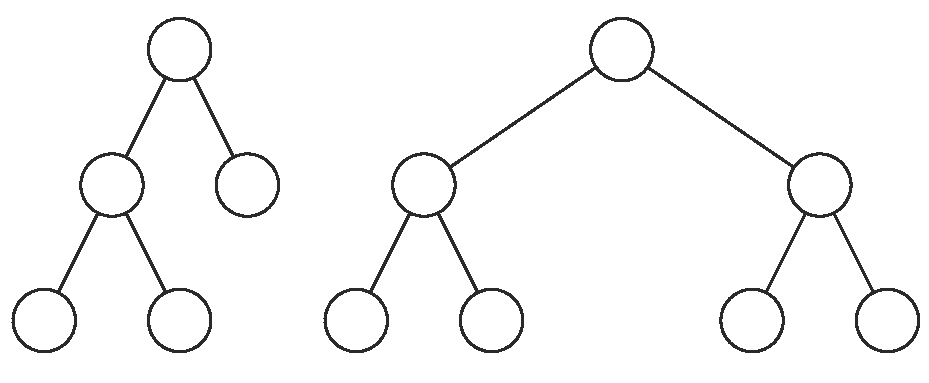
\includegraphics[width=0.85\linewidth]{figures/cutting/BVH.png}
  \caption{---}\label{fig:BVH_flow}
\end{figure}


\begin{figure}
  \centering%
  \includegraphics[width=0.85\linewidth]{figures/cutting/Process_cut_details.png}
  \caption{---}\label{fig:Process_cut_details_flow}
\end{figure}


\begin{figure}
  \centering%
  \includegraphics[width=0.85\linewidth]{figures/cutting/cuttetrahedron.png}
  \caption{---}\label{fig:CutTetrahedron_flow}
\end{figure}


\begin{figure}
  \centering%
  \includegraphics[width=0.85\linewidth]{figures/cutting/subdivision.png}
  \caption{---}\label{fig:Subdivision_flow}
\end{figure}


\subsubsection{Enhanced Cutting Operations}

\textbf{Adaptive Cutting}\\

\textbf{Mesh Cleanup and Simplification}\\
Once the cut is processed and the mesh updates are done, a further post-process first cleans the mesh of any flat cells and reduces the number of new cells. The mesh simplification algorithm maintains a good mesh topology without cell inversions, a problem that is usually hard to solve globally, it also maintains the geometry of the cut on the mesh as well as the mesh volume for maximum visual fidelity on all levels.

The algorithm operates by iterating on edge contractions. An edge contraction operation on edge $ij$ removes vertex $j$ and reattaches to $i$ all tetrahedra that were incident to $j$. Edge contraction follows an order based on the priority of vertices. Vertices on the cutting surface are of highest priority and are not removed in order to preserve the shape of the cut. Vertices in the interior of the volume have lowest priority and are removed first to simplify the mesh. Vertices on the boundary are next in the priority and are removed as needed to simplify the model while keeping the original volume intact.
